% ---------------------------------------------------------------------------
% ACT D (COMPRESSIBLE MULTIPOINT) -- ONE SHAPE, THREE ANGLES, COMPRESSIBLE.
% One-page customer-facing result sheet for the D19M NACA0012 COMPRESSIBLE
% alpha-multipoint SHAPE OPTIMISATION.
% Compile: pdflatex ACT_D_compressible_multipoint_sheet.tex
%
% ---------------------------------------------------------------------------
% WHY THIS IS A SEPARATE SHEET AND NOT A PAGE, COLUMN OR ROW OF THE
% INCOMPRESSIBLE ONE.  Four measured reasons, not a preference:
%
%   1. DIFFERENT PHYSICS, DIFFERENT REYNOLDS NUMBER BY AN ORDER OF MAGNITUDE.
%      The SO-3 sheet is DASimpleFoam, incompressible, U = 10 m/s, nu 1.5e-5,
%      Re 6.67e5.  THIS is DARhoSimpleFoam, compressible, U = 100 m/s,
%      mu 1.8e-5, rho 1.1769, Re 6.54e6 and M 0.288.  A shared table would put
%      two Reynolds numbers a factor of ten apart under one header.
%   2. DIFFERENT OPERATING POINTS.  SO-3 registers 3.139 / 5.139 / 7.139 deg
%      about the INCOMPRESSIBLE tutorial's trimmed angle.  This item registers
%      2.787333582 / 4.787333582 / 6.787333582 about D19O's OWN measured
%      compressible trimmed angle at CL_target = 0.5.  The two triples are not
%      the same condition and must never be read down one column.
%   3. THE VERDICTS ARE NOT THE SAME CLASS.  SO-3's item verdict is PASS.  This
%      item's is GATE REACHED on both rows: both compose PASS and both are
%      CAPPED by a ceiling REGISTERED BEFORE THE RUN.  On one sheet the ceiling
%      would inevitably render as a qualification on a shared table, which is
%      the footnote failure this sheet exists to avoid.
%   4. THE SO-3 SHEET HAS NO VERTICAL SLACK.  Its own header block records that
%      a single extra table row pushed it to two pages and that the body
%      leading had to drop from 8.5 to 8.0 to buy 28pt.  There is no room to
%      merge and no honest way to make room.
%
% THE HEAD RULE OF THIS FAMILY IS UNCHANGED AND THIS SHEET OBEYS IT: several
% different subjects are called "Act D" and THEIR NUMBERS MUST NEVER BE MERGED.
%   ACT_D_aerofoil_section_sheet.tex      2D NACA0012, SO-3aR2, NO OPTIMISER RAN
%   ACT_D_reference_wing_sheet.tex        3D reference wing, 38,304 cells
%   ACT_D_multipoint_optimisation_sheet   2D NACA0012, SO-3, INCOMPRESSIBLE
%   THIS SHEET                            2D NACA0012, D19M, COMPRESSIBLE
% This sheet supersedes nothing.  It is a sibling, not a successor.
%
% ---------------------------------------------------------------------------
% WHICH ROW IS ON CAMERA.  The item grades TWO rows, SHIPPED and PATCHED, on
% two builds of the mesh deformation library.  Both are GATE REACHED, both
% compose verdict_before_ceiling = PASS.  THIS SHEET CARRIES THE PATCHED ROW,
% because a demo shows ONE run and which library build produced it is METHOD,
% which the demo may withhold.  It may never misstate a RESULT, and it does
% not.  The two rows are NOT a repeatability pair and are not shown as one.
% Table 6 states that both builds run and gives their combined measured cost,
% so no reader can take this run's own 17.650 core-min for the item's total.
%
% ---------------------------------------------------------------------------
% THE CEILING, AND WHY IT IS A BAND ACROSS THE TOP OF THE FACE RATHER THAN A
% FOOTNOTE.  Verbatim from the frozen grade file's `verdict_ceiling_reason`:
%
%   "The compressible single-point gradient this optimisation spends has NO
%    GRADED VERDICT (D19R's grader refused rc=2; D19R2 grading attempt 1 = NOT
%    A RESULT) and its plateau did NOT close (all_two_sided=false,
%    score_pct=21.060684242435336, binding=[shape[7],CD,fine]).
%    DAFOAM_CHARTER.md section 1: a gradient is not a result until an FD table
%    stands beside it at a step PROVED to lie in the plateau.  This item
%    therefore cannot publish PASS on any row or at item level, whatever its
%    gates return.  REGISTERED BEFORE THE RUN."
%
% ACCURACY POINT THAT AN EARLIER DRAFT OF THIS BLOCK GOT WRONG AND THAT THE
% FACE MUST NOT REPEAT: the 21.0607 % figure is D19R's measurement at the
% BASELINE shape, on shape[7]/CD, on the fine side of s* = 1e-3.  IT IS NOT A
% MEASUREMENT MADE IN THIS RUN.  In THIS run shape[7]'s own J plateau is
% two-sided and scores 2.9438 % against a 10 % tolerance
% (gates.G-PLAT7.PATCHED.components.shape[7].plateau_J).  shape[7] is excluded
% here NOT because it fails here but because it is a REGISTERED NON-RESULT,
% named before the run, carried forward unchanged from D19O, WHATEVER VALUE IT
% RETURNS.  The face therefore says the control is set aside beforehand and
% counts in no total, and says nothing about a 21 % reading it did not take.
%
% NO VERDICT TOKEN REACHES THE RENDERED FACE.  `GATE REACHED`, `PASS`, `NOT A
% RESULT`, the row names and the library-build names are all off camera.  The
% ceiling is rendered as what it IS to a customer: a statement of what this
% sheet does not claim.
%
% ---------------------------------------------------------------------------
% PROVENANCE OF EVERY USER-VISIBLE NUMBER (not rendered; for the lab only).
% Run root:
%   /home/ubuntu/certonomous-runs/
%     CURRICULUM-D19M-a1-naca0012-subsonic-multipoint/
% Frozen grade file (item GATE REACHED, rows SHIPPED / PATCHED both GATE
% REACHED, both verdict_before_ceiling PASS):
%   D19M_grade_20260901T083034Z.json,  graded 2026-09-01T08:30:34Z
% Producer:  cases/dafoam/ladder-a/A1/curriculum_D19M/d19m_runScript.py
%
%   TABLE 1 operating condition, all from the producer's PHYSICS BLOCK
%   (d19m_runScript.py lines 88-95, 100-132) and MESH/constant/
%   thermophysicalProperties:
%     U0 = 100.0 m/s, p0 = 101325.0 Pa, T0 = 300.0 K, nuTilda0 = 4.5e-5,
%     A0 = 0.1 m^2, chord 1 m, rho0 = p0/T0/287 = 1.1768873 kg/m^3
%     mu = 1.8e-5 Pa s, Pr = 0.7, Cp = 1005, molWeight 28.97  [thermophysical]
%     solver DARhoSimpleFoam (daOptions solverName), turbulence SpalartAllmaras
%     nu = mu/rho = 1.52947e-5 m^2/s  ->  Re = U c / nu = 6.5382e6  -> 6.54e6
%     R = 8314.47/28.97 = 286.99;  Cv = Cp - R = 718.0;  gamma = 1.39972
%     a = sqrt(gamma R T) = 347.15 m/s  ->  M = 100/347.15 = 0.2880
%     THE MACH ROW IS DERIVED FROM THE CASE'S OWN Cp AND molWeight, not from an
%     assumed speed of sound.  This is STRONGER than the SO-3 sheet's Mach row,
%     which assumes 340 m/s, and the difference is stated rather than blurred.
%     alphas 2.787333582 / 4.787333582 / 6.787333582 deg and weights 1/3 each,
%       tolerance 1e-12, read back with abs_err 0.0 on ALL FIVE arms
%       (gates.G-ALPHA.per_arm: MESH is not an arm here; O-S O-P XE-P FE-S FE-P)
%     mesh 4032 cells: gates.G-M2_mesh_identity {cells 4032, registered 4032}
%
%   THE GRID AND THE FFD ARE THE SAME ARTEFACTS AS SO-3's, AND THAT IS
%   MEASURED, NOT ASSUMED.  md5 over both run roots, this lane, 2026-09-01:
%     points.gz    38a486d29a540ecd1b06e006e66475e7   IDENTICAL
%     faces.gz     5982fd363aef3df745d9059ddbc009af   IDENTICAL
%     owner.gz     9d601f4f3174da4c8f8b41d4100ace17   IDENTICAL
%     neighbour.gz d8c6c5b6d45b6e93b50704151c3c832c   IDENTICAL
%     boundary     c92a945e9a1405b988ab418e48ab53c3   IDENTICAL
%     wingFFD.xyz  6ddf378b028d03d8a18270488bee1759   IDENTICAL
%   SO the far-field radius 18.583 m, the first-layer height 2.0629e-03 to
%   4.0659e-03 m and the 126 wall nodes measured off SO-3's polyMesh by
%   cases/dafoam/render_so3_mesh_figures.py are measurements OF THIS RUN'S OWN
%   GRID, byte for byte, and Figure 1 is a true picture of it.
%   FOLLOW-ON OWED AND NAMED RATHER THAN QUIETLY SKIPPED: a D19M-named render
%   from D19M's own run root, so the figure's provenance does not rest on a
%   hash comparison a later reader has to repeat.  Until that exists this block
%   IS the provenance and the hashes above are the evidence.
%
%   TABLE 2 result, PATCHED row, gates.G-OPT9.PATCHED:
%     CD_baseline [0.012653042938099815, 0.0163267535192322,
%                  0.02295234328709633]
%     CD_final    [0.011620047210203866, 0.012051987264322876,
%                  0.014765583462742194]
%     CL_baseline [0.2987459621941071, 0.49999949596851295,
%                  0.6736631644915069]
%     CL_final    [-0.15737009883292363, 0.07216486641740512,
%                  0.305403456283111]
%     J_baseline 0.017310713248142783   J_final 0.012812539312422978
%     weighted_drag_reduction_pct 25.98491391567821
%
%   THE 25.985 % IS NEVER ON THIS FACE WITHOUT THE THREE-CL TRIPLE IN THE SAME
%   FRAME.  The grade file states the rule itself, verbatim, at
%   gates.G-OPT9.<ROW>._cl_travels:
%     "CL is UNCONSTRAINED here -- alpha is the operating point, so there is no
%      DV to trim with.  THE THREE-CL TRIPLE therefore travels with every
%      weighted-drag number this item publishes.  A reduction at unstated lift
%      is not a reportable number."
%   It appears in exactly three places on the face and each one carries the
%   lift beside it: the headline paragraph (which states the negative value),
%   Table 2 (whose CL start and CL final columns are the same table), and
%   Figure 2 (whose second panel is the lift collapse).  It appears nowhere
%   else.  check_actD_compressible_sheet_face.py enforces this on the RENDERED
%   face, in both directions, with planted controls.
%
%   AND gates.G-OPT9.<ROW>._improvement_grades_nothing, verbatim:
%     "DAFOAM_CHARTER.md section 9 forbids grading an optimisation by the size
%      of its improvement.  `drag_reduction_pct` is reported and is an input to
%      the REGISTERED intermediate threshold only."
%   Registered intermediate threshold 2.0 %; registered minimum majors 5.
%
%   TABLE 3 optimiser, gates.G-OPT9.PATCHED:
%     IPOPT; ipopt_n_iterations 10; ipopt_table_rows 11; max_iter_registered
%     40; reached_iteration_cap false; ipopt_exit "Optimal Solution Found.";
%     ipopt_printed_convergence true; stall_condition_A null;
%     stall_condition_B_state "NOT EXERCISED"
%   NO OBJECTIVE-PER-MAJOR TRACE IS ON THIS SHEET, AND THE ABSENCE IS
%   DELIBERATE.  The frozen grade file carries no per-major objective series
%   for this item (checked: gates.G-OPT9.<ROW> has no such key), so drawing the
%   descent would mean a lane parsing the IPOPT log by hand.  A number read by
%   an instrument that has not been shown able to see a planted false value is
%   not evidence (CLAUDE.md rule 3).  The cost of the figure is therefore a
%   build_d19m_demo_series.py with a planted reader control, modelled on
%   build_so3_demo_series.py; it is named here as OWED rather than approximated.
%
%   TABLE 4 endpoint gradient, PATCHED row, gates.G5_fd.PATCHED, quantity J,
%   graded_components ["shape[0]","shape[3]","shape[6]"], band_D = band_E =
%   5.0 %, min_graded_components 3, n_graded_components 3, fe_arm FE-P:
%     shape[0] adjoint -0.003382200437339747  fd -0.0033768259902981074
%              rel 0.15915676606022539 %   plateau two-sided
%     shape[3] adjoint  0.0025079828176175108 fd  0.0025097542272816895
%              rel 0.07058100131570638 %   plateau two-sided
%     shape[6] adjoint -0.018663528794594746 fd -0.018662319758074204
%              rel 0.006478490006683075 %  plateau two-sided
%     aggregate_pct_excl_flagged_J  0.030247524615185435
%     aggregate_pct_excl_flagged_CL 0.018669889179977413
%   SHIPPED row for the record and NOT on the face: J 0.046572281721388005,
%   CL 0.019347138573858103.
%   EXCLUDED BY NAME, gates.G5_fd.PATCHED.excluded_from_aggregate [["shape",7]]:
%     shape[7], the trailing-edge pair, REGISTERED BEFORE THE RUN as a
%     NON-RESULT on the plateau clause, on BOTH rows, WHATEVER VALUE IT
%     RETURNS, carried forward unchanged from D19O.
%   THE HARNESS-SOUND FLOOR IS REPORTED AND NEVER GATED, and the grade file
%   says so itself at gates.G5_fd.<ROW>._harness_floor:
%     "VERIFICATION_CHARTER.md section 7 step 4: the harness-sound floor on
%      this stack is 2.5 to 5 % vector-norm relative error, and a number below
%      that is a claim about the harness.  REPORTED, NEVER GATED."
%     harness_floor_pct [2.5, 5.0].  Every agreement figure in Table 4 lies
%     BELOW that floor, so the face says the claim is the five per cent limit
%     and not the digit, and says the floor is reported rather than used.
%   Control-name map, from base/FFD/wingFFD.xyz (5x2x2, x stations -0.010,
%   0.245, 0.500, 0.755, 1.010; y +/-0.070) and the shape construction at
%   d19m_runScript.py:237-246, which is UNCHANGED from D19O's producer:
%     interior i=1,2,3 with j=0 lower / j=1 upper give indices 0..5 in order;
%     i=0 and i=4 give the two symmetric edge pairs as indices 6 and 7.
%     shape[0] lower surface x/c = 0.245   shape[3] upper surface x/c = 0.500
%     shape[6] leading-edge pair           shape[7] trailing-edge pair
%
%   MULTIPOINT ASSEMBLY IDENTITY, gates.G-MP-STRUCT.PATCHED: dJ == sum_w dCD
%   over all 8 components, worst_rel 7.867135428691222e-12 against rtol 1e-10.
%   SHIPPED worst_rel 4.254668614780759e-12.  xe_arm XE-P.
%
%   TABLE 5 instrument checks, from `controls` and gates.G-TB.PATCHED:
%     R3_read_mesh_cells: on disk 4032, planted 4039, read_back 4039, seen true
%     R5_read_X: plant 0.001234 over 56 values, worst residual 1.7932703932910243e-16
%     R6_read_F: plant 0.001234 over 64 values, worst residual 1.7932703932910243e-16
%       -> the face says "120 values" and "2e-16", which is 56 + 64 and the
%          worst of the two residuals, not an average of anything
%     R8_read_alphas: unplanted_first 2.787333582, plant_deg 1.0,
%       planted_first 3.787333582, seen true
%     R1_read_ledger: unplanted 6.383, planted 6.384234, read_back 6.384234
%     G-TB (deliberately unsuitable step 1e-8, five orders below s*):
%       0 of 3 components pass band D; shape[0] 109.74 %, shape[3] 90.61 %,
%       shape[6] 52.26 %.  max_passing 1, n_passing 0.
%     birth_register: 9 readers, 9 born, 0 not born, 6 of them can pass a gate
%       on a zero.
%
%   TABLE 6 compute, from gates.G10_caps.per_arm and the run root's ledger.txt
%   ARM= rows, ranks=1 on every arm (gates.G-NP registered 1 for all seven), so
%   core-min = wall s / 60 exactly:
%     PATCHED path, the run on this sheet:
%       MESH  0.167 core-min (10 wall s)   predicted 0.20   ratio 0.835
%       O-P   8.083 core-min (485 wall s)  predicted 8.64   ratio 0.9355
%       XE-P  3.017 core-min (181 wall s)  predicted 2.60   ratio 1.1604
%       FE-P  6.383 core-min (383 wall s)  predicted 5.71   ratio 1.1179
%       path total 17.650 core-min, 1059 wall s
%       dollars 17.650/60*0.0513 = 0.0150911 -> $0.0151 DERIVED, NOT MEASURED
%     WHOLE ITEM, both builds, all seven arms:
%       total_core_min 35.166, 2110 wall s, usd_derived_not_measured 0.030067
%       item_point_prediction_core_min 34.10, ratio_actual_over_predicted_item
%       1.0313, item_ceiling_core_min 149.0, arms_over_cap [], total_over_
%       ceiling false
%   THE PREDICTED COLUMN AND THE RATIO ARE OFF THE RENDERED FACE.  A PREDICTION
%   MUST NEVER STAND ON CAMERA AS WHAT THE RUN COST.  That exact defect was
%   caught on this act once already, in four places rather than one.  The rule-
%   12 estimate-versus-actual comparison is NOT lost by keeping it off camera:
%   it belongs in this item's row in docs/COST_CALIBRATION.md, and THAT ROW IS
%   NOT YET FILED -- reported here as OWED, and it is not a lane's to file
%   silently.  Every figure on the face is a reading from this item's clock.
%   Cost basis: c7a.4xlarge at $0.0513/core-h, REPORTED-BY-OWNER 2026-08-21/22,
%   NOT MEASURED -- the box cannot read its own billing (COMPUTE_BUDGET_CHARTER
%   section 5).  Core-minutes ARE measured.
%
%   THE TWENTY-MINUTE DISPLAY FIGURE.  A standing capture directs the dafoam
%   demo to show 20 minutes rather than 60.  It attaches to a 3601 s figure on
%   the reference-wing act.  THIS run's own PATCHED path is 1059 wall s, 17.7
%   minutes, already under twenty; the whole item is 2110 wall s, 35.2 minutes,
%   which is OVER twenty and is on the face as the item figure and never as
%   this run's.  No time figure here is invented.  Whether the 20-minute
%   display figure extends to this act is not a lane's call and is referred.
%
%   ASSUMED, NOT MEASURED, and kept out of every measured table:
%     y+ about 250 to 490, estimated as u_tau*y/nu with y half the measured
%       first-layer height and cf = 0.026 Re^(-1/7) (flat-plate correlation):
%       cf = 0.002761, tau_w = 16.25 Pa, u_tau = 3.716 m/s,
%       y = 1.03e-3 to 2.03e-3 m, nu = 1.52947e-5.
%       THE RUN WRITES NO y+ FIELD, so this is a correlation, never a reading.
%       IT IS AN ORDER OF MAGNITUDE ABOVE THE SO-3 SHEET'S 30 TO 60 BECAUSE U
%       IS TEN TIMES HIGHER ON THE SAME GRID, and the face says so, because a
%       reader who carries the incompressible sheet's y+ range across would be
%       wrong by a factor of eight.
%
% ---------------------------------------------------------------------------
% BINDING CAPTURES THIS SHEET IS WRITTEN TO (not rendered).
%   Act A figure and header standard: header carries the solver line of the
%   source run; figures carry no paragraphs; title at most 10 words; axis
%   labels with units; legend inside the axes; one caption line of at most 20
%   words; explanation moves to the sheet text; sheet paragraphs at most 3
%   sentences.
%   Demo mode: every number, field and figure is the real run's; present-tense
%   solved-case wording; no replay, storage or substitution language anywhere.
%   Overnight order: live-looking, synchronized, no internal information, no
%   past tense, short sentences, all results in tables, real geometry and its
%   real mesh only, professional prompts, all plots latexified.
%   Standing product rules: repeated per-item numbers are always a table; every
%   plot self-explanatory; name the reference area for any coefficient; state
%   the finite-difference step AND that it was swept; y+ range and wall
%   treatment on the mesh table; measured and assumed never share a table
%   header; no dashes on a camera surface; no repository paths on camera.
% ---------------------------------------------------------------------------
\documentclass[9pt,a4paper]{article}
\usepackage[margin=8mm,top=4mm,bottom=1mm]{geometry}
\usepackage{booktabs}
\usepackage{array}
\usepackage{xcolor}
\usepackage{graphicx}
\usepackage{amssymb}
\usepackage[T1]{fontenc}

\definecolor{band}{rgb}{0.87,0.91,0.96}
\definecolor{accent}{rgb}{0.10,0.32,0.60}
\definecolor{warm}{rgb}{0.72,0.30,0.06}
\definecolor{rulegrey}{rgb}{0.45,0.45,0.45}
\definecolor{boxgrey}{rgb}{0.96,0.96,0.94}
\definecolor{limitgrey}{rgb}{0.93,0.92,0.89}

\renewcommand{\footnotesize}{\fontsize{6.4}{6.85}\selectfont}
\renewcommand{\scriptsize}{\fontsize{5.7}{6.1}\selectfont}
\renewcommand{\arraystretch}{0.92}
\setlength{\parindent}{0pt}
\setlength{\parskip}{0pt}
\setlength{\tabcolsep}{3.2pt}
\pagestyle{empty}

\newcommand{\rolesig}[1]{\textbf{\footnotesize#1}}
\graphicspath{{../../../cases/dafoam/ladder-a/figures/}}

\fontsize{7.3}{8.0}\selectfont

\begin{document}
\fontsize{7.3}{8.0}\selectfont

% ---------------------------------------------------------------- title -----
{\fontsize{13.5}{15}\selectfont\bfseries One shape, three angles, compressible}\\[1.5pt]
{\fontsize{8.6}{10}\selectfont Gradient driven shape optimisation of a
NACA0012 section, compressible, steady, two dimensional}\\[2pt]
{\color{rulegrey}\rule{\textwidth}{0.9pt}}\\[1pt]
{\footnotesize \textbf{Solver: DAFoam \texttt{DARhoSimpleFoam}, steady
compressible RANS, Spalart-Allmaras turbulence, discrete adjoint, IPOPT.}
Your request: \emph{minimise the drag of this section averaged over three
angles of attack, $2.787$, $4.787$ and $6.787$ degrees, weighted equally, at
$100\,\mathrm{m\,s^{-1}}$; one shape serves all three; verify the gradient at
the final shape.}}

% ------------------------------------------------------- the ceiling band ---
\vspace{1.5pt}
\colorbox{limitgrey}{\begin{minipage}{0.985\textwidth}
\vspace{1pt}
{\footnotesize\textbf{What this sheet does not claim, fixed before the run and
not after it.}
$\bullet$ The compressible gradient this optimiser spends carries no separate
check of its own on this section; what stands here is one check, at the final
shape, on three of the eight shape controls.
$\bullet$ The trailing edge control is set aside by name before this run
starts, on both builds, whatever value it returns, and counts in no total here.
$\bullet$ The size of an improvement grades nothing here and is never what
this run stands on.}
\vspace{1pt}
\end{minipage}}

% ================================================================= row 1 =====
\vspace{1.5pt}
\begin{minipage}[t]{0.505\textwidth}
\textbf{What the optimiser does, and what it costs you}

\vspace{1pt}
{\footnotesize \textbf{Lift carries no constraint here and the optimiser spends
it.} The weighted drag objective falls $25.985$ per cent and lift falls with
it, from $0.29875$, $0.50000$, $0.67366$ to $\mathbf{-0.15737}$, $0.07216$,
$0.30540$: negative at the lowest angle. The optimiser stops on its own
statement, not on the iteration cap.\\[2pt]
\textbf{What this run establishes.} The gradient driving the descent is checked
against an independent calculation \emph{at the final shape}, on three
controls, and agrees to $0.16$ per cent against a five per cent limit fixed
beforehand. The optimiser and that check agree; the section is not a better
aerofoil.}

\vspace{1.5pt}
\textbf{Table 1. Operating condition and grid.}

\vspace{1.5pt}
{\fontsize{6.7}{7.9}\selectfont
\begin{tabular}{@{}l r l l@{}}
\toprule
Quantity & Value & Unit & Basis \\
\midrule
Freestream speed $U$          & $100$               & m\,s$^{-1}$     & exact input \\
Static pressure $p$           & $101\,325$          & Pa              & exact input \\
Static temperature $T$        & $300$               & K               & exact input \\
Dynamic viscosity $\mu$       & $1.8\times10^{-5}$  & Pa\,s           & exact input \\
Chord $c$                     & $1$                 & m               & exact input \\
Reference area $A$            & $0.1$               & m$^2$           & exact input \\
Reynolds number $Uc/\nu$      & $6.54\times10^{6}$  &                 & derived \\
Mach number                   & $0.288$             &                 & derived \\
Angles $\alpha$               & $2.787$, $4.787$, $6.787$ & deg       & registered \\
Weights                       & $1/3$ each          &                 & registered \\
\midrule
Grid                          & $4\,032$            & cells           & counted \\
Far field radius              & $18.6$              & m               & measured \\
First layer height            & $2.06$ to $4.07$    & $10^{-3}$ m     & measured \\
\bottomrule
\end{tabular}}

\vspace{1pt}
{\scriptsize The angles and weights read back with zero deviation at
$10^{-12}$. Density $1.1769\,\mathrm{kg\,m^{-3}}$ and Mach follow from the
case's own heat capacity and molecular weight. The wall treatment is a
continuous wall function valid across the whole near-wall range, and
coefficients are formed on the reference area above.}
\end{minipage}\hfill
\begin{minipage}[t]{0.475\textwidth}
\textbf{Figure 1. The grid the section is solved on.}

\vspace{1.5pt}
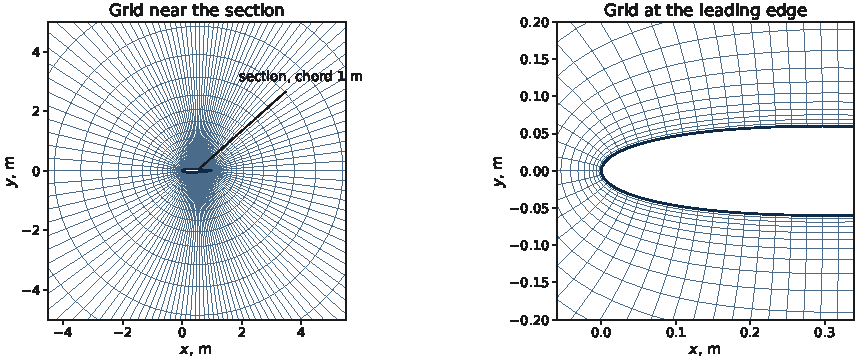
\includegraphics[width=0.76\textwidth]{so3_grid_pair.pdf}

\vspace{0.5pt}
{\scriptsize All $4\,032$ cells are drawn. The left view stops at about
$5\,\mathrm{m}$; the far field radius is $18.6\,\mathrm{m}$.}

\vspace{2pt}
\textbf{Table 2. The result. Drag falls and lift collapses.}

\vspace{1.5pt}
{\fontsize{6.7}{7.9}\selectfont
\begin{tabular}{@{}r r r r r@{}}
\toprule
$\alpha$, deg & $C_D$ start & $C_D$ final & $C_L$ start & $C_L$ final \\
\midrule
$2.787$ & $0.012653$ & $0.011620$ & $0.29875$ & $\mathbf{-0.15737}$ \\
$4.787$ & $0.016327$ & $0.012052$ & $0.50000$ & $0.07216$ \\
$6.787$ & $0.022952$ & $0.014766$ & $0.67366$ & $0.30540$ \\
\midrule
Weighted $J$ & $0.0173107$ & $0.0128125$ & & \\
\bottomrule
\end{tabular}}

\vspace{1.5pt}
{\scriptsize $J$ is the equally weighted mean of the three drag coefficients
and it falls by $25.985$ per cent. Every lift coefficient falls with it and one
turns negative, so the drag figure is never quoted apart from these lift
columns.}
\end{minipage}

% ================================================================= row 2 =====
\vspace{2pt}
{\color{rulegrey}\rule{\textwidth}{0.5pt}}\\[1pt]
\begin{minipage}[t]{0.50\textwidth}
\textbf{Figure 2. Drag and lift at three angles of attack.}

\vspace{2pt}
\setlength{\unitlength}{1mm}
\begin{picture}(72,27)(-7.5,-6.5)
  % ---------------- panel A: C_D -------------------------------------------
  \linethickness{0.4pt}
  \put(0,0){\line(1,0){27}}
  \put(0,0){\line(0,1){20}}
  \multiput(0,2.857)(0,5.714){4}{\line(-1,0){1.1}}
  \put(-1.7,2.057){\makebox(0,0)[r]{\scriptsize $0.012$}}
  \put(-1.7,7.771){\makebox(0,0)[r]{\scriptsize $0.016$}}
  \put(-1.7,13.486){\makebox(0,0)[r]{\scriptsize $0.020$}}
  \put(-1.7,19.200){\makebox(0,0)[r]{\scriptsize $0.024$}}
  \put(-6.6,10){\makebox(0,0)[c]{\rotatebox{90}{\scriptsize $C_D$}}}
  \multiput(3,0)(6,0){5}{\line(0,-1){1.1}}
  \put(3,-3.1){\makebox(0,0)[c]{\scriptsize $3$}}
  \put(9,-3.1){\makebox(0,0)[c]{\scriptsize $4$}}
  \put(15,-3.1){\makebox(0,0)[c]{\scriptsize $5$}}
  \put(21,-3.1){\makebox(0,0)[c]{\scriptsize $6$}}
  \put(27,-3.1){\makebox(0,0)[c]{\scriptsize $7$}}
  \put(13.5,-5.6){\makebox(0,0)[c]{\scriptsize $\alpha$, deg}}
  \linethickness{0.5pt}
  {\color{accent}\qbezier(1.722,3.790)(7.722,6.415)(13.722,9.039)
   \qbezier(13.722,9.039)(19.722,13.771)(25.722,18.503)
   \put(1.722,3.790){\circle*{1.1}}\put(13.722,9.039){\circle*{1.1}}
   \put(25.722,18.503){\circle*{1.1}}}
  {\color{warm}
   \multiput(1.722,2.314)(1.500,0.077){8}{\rule{0.9mm}{0.4pt}}
   \multiput(13.722,2.931)(1.500,0.485){8}{\rule{0.9mm}{0.4pt}}
   \put(1.022,1.614){\framebox(1.4,1.4){}}
   \put(13.022,2.231){\framebox(1.4,1.4){}}
   \put(25.022,6.109){\framebox(1.4,1.4){}}}
  \put(2.6,18.8){\makebox(0,0)[l]{\scriptsize\color{accent}$\bullet$\ start}}
  \put(2.6,16.3){\makebox(0,0)[l]{\scriptsize\color{warm}$\square$\ final}}
  % ---------------- panel B: C_L -------------------------------------------
  \put(40,0){
    \linethickness{0.4pt}
    \put(0,0){\line(1,0){27}}
    \put(0,0){\line(0,1){20}}
    {\color{rulegrey}\multiput(0,4.444)(3,0){9}{\rule{1.7mm}{0.3pt}}}
    \multiput(0,0)(0,4.444){5}{\line(-1,0){1.1}}
    \put(-1.7,-0.8){\makebox(0,0)[r]{\scriptsize $-0.2$}}
    \put(-1.7,3.644){\makebox(0,0)[r]{\scriptsize $0.0$}}
    \put(-1.7,8.089){\makebox(0,0)[r]{\scriptsize $0.2$}}
    \put(-1.7,12.533){\makebox(0,0)[r]{\scriptsize $0.4$}}
    \put(-1.7,16.978){\makebox(0,0)[r]{\scriptsize $0.6$}}
    \put(-6.2,10){\makebox(0,0)[c]{\rotatebox{90}{\scriptsize $C_L$}}}
    \multiput(3,0)(6,0){5}{\line(0,-1){1.1}}
    \put(3,-3.1){\makebox(0,0)[c]{\scriptsize $3$}}
    \put(9,-3.1){\makebox(0,0)[c]{\scriptsize $4$}}
    \put(15,-3.1){\makebox(0,0)[c]{\scriptsize $5$}}
    \put(21,-3.1){\makebox(0,0)[c]{\scriptsize $6$}}
    \put(27,-3.1){\makebox(0,0)[c]{\scriptsize $7$}}
    \put(13.5,-5.6){\makebox(0,0)[c]{\scriptsize $\alpha$, deg}}
    \linethickness{0.5pt}
    {\color{accent}\qbezier(1.722,11.083)(7.722,13.319)(13.722,15.556)
     \qbezier(13.722,15.556)(19.722,17.485)(25.722,19.415)
     \put(1.722,11.083){\circle*{1.1}}\put(13.722,15.556){\circle*{1.1}}
     \put(25.722,19.415){\circle*{1.1}}}
    {\color{warm}
     \multiput(1.722,0.947)(1.500,0.638){8}{\rule{0.9mm}{0.4pt}}
     \multiput(13.722,6.048)(1.500,0.648){8}{\rule{0.9mm}{0.4pt}}
     \put(1.022,0.247){\framebox(1.4,1.4){}}
     \put(13.022,5.348){\framebox(1.4,1.4){}}
     \put(25.022,10.531){\framebox(1.4,1.4){}}}
    \put(3.4,2.6){\makebox(0,0)[l]{\scriptsize lift $=-0.157$ here}}
    \put(15.3,17.2){\makebox(0,0)[l]{\scriptsize\color{accent}$\bullet$\ start}}
    \put(15.3,14.7){\makebox(0,0)[l]{\scriptsize\color{warm}$\square$\ final}}
  }
\end{picture}

\vspace{1pt}
{\scriptsize Lift falls at every angle and turns negative at the lowest, which
is the price of the $25.985$ per cent drag reduction.}

\vspace{2pt}
\textbf{Table 3. The optimiser.}

\vspace{1.5pt}
{\fontsize{6.7}{7.9}\selectfont
\begin{tabular}{@{}l r@{}}
\toprule
Quantity & Value \\
\midrule
Optimiser                                & IPOPT \\
Major iterations taken                   & $10$ \\
Iteration cap, fixed beforehand          & $40$ \\
Minimum majors, fixed beforehand         & $5$ \\
Improvement threshold, fixed beforehand  & $2$ per cent \\
Terminal statement                       & Optimal Solution Found. \\
\bottomrule
\end{tabular}}

\vspace{1pt}
{\scriptsize The optimiser prints its own convergence statement and stops a
quarter of the way into its budget. The improvement threshold is an input it
must clear, never the thing this run stands on.}
\end{minipage}\hfill
\begin{minipage}[t]{0.475\textwidth}
\textbf{Table 4. The gradient, checked at the final shape.}

\vspace{1.5pt}
{\fontsize{6.7}{7.9}\selectfont
\begin{tabular}{@{}l r r r@{}}
\toprule
Shape control & Computed & Checked &
  \begin{tabular}{@{}r@{}}Difference,\\ \% of checked\end{tabular} \\
\midrule
Lower surface, $x/c=0.245$ & $-0.003382$ & $-0.003377$ & $\mathbf{0.159}$ \\
Upper surface, $x/c=0.500$ & $+0.002508$ & $+0.002510$ & $0.071$ \\
Leading edge pair          & $-0.018664$ & $-0.018662$ & $0.006$ \\
\midrule
\multicolumn{3}{@{}l}{All three together, on the objective} & $0.030$ \\
\multicolumn{3}{@{}l}{All three together, on lift}          & $0.019$ \\
\multicolumn{3}{@{}l}{Limit, fixed before the run}          & $5.00$ \\
\midrule
\multicolumn{4}{@{}l}{\emph{Trailing edge pair: set aside by name before the
run, in no total here}} \\
\bottomrule
\end{tabular}}

\vspace{1pt}
{\scriptsize Values are per metre of control travel and chord is
$1\,\mathrm{m}$. The step is swept over three sizes and the figure quoted is
the middle one, where the estimate stops moving, at the shape the optimiser
returns rather than the one it starts from.}

\vspace{1pt}
{\scriptsize \textbf{Agreement finer than two and a half to five per cent is at
the resolution of the comparison itself, and is never used as a limit}, so the
claim is the five per cent limit and not the digits above.}

\vspace{2pt}
\textbf{Table 5. Instrument checks.}

\vspace{1.5pt}
{\fontsize{6.7}{7.9}\selectfont
\begin{tabular}{@{}l r@{}}
\toprule
Check & Result \\
\midrule
Planted grid count, $4\,039$          & read back \\
Planted zero, $120$ values            & $2\times10^{-16}$ \\
Planted angle, one degree adrift      & read back \\
Planted cost row, $6.384$ core-min    & read back \\
Deliberately wrong step, 3 controls   & $0$ pass \\
Weighted sum identity, 8 controls     & $8\times10^{-12}$ \\
\bottomrule
\end{tabular}}

\vspace{1pt}
{\scriptsize Each reader is shown a known false value before it is trusted, and
each one sees it. Driven at a deliberately unsuitable step, the gradient check
fails on every control, by $52$ to $110$ per cent.}
\end{minipage}

% ================================================================= row 3 =====
\vspace{2pt}
{\color{rulegrey}\rule{\textwidth}{0.5pt}}\\[1pt]
\begin{minipage}[t]{0.335\textwidth}
\textbf{Table 6. Compute: what this run costs.}

\vspace{1.5pt}
{\fontsize{6.7}{7.9}\selectfont
\begin{tabular}{@{}l r r@{}}
\toprule
Stage & \begin{tabular}{@{}r@{}}Cost,\\ core-min\end{tabular}
      & \begin{tabular}{@{}r@{}}Wall clock,\\ s\end{tabular} \\
\midrule
Geometry and grid           & $0.167$  & $10$ \\
Optimisation, 10 majors     & $8.083$  & $485$ \\
Endpoint gradient           & $3.017$  & $181$ \\
Independent check of it     & $6.383$  & $383$ \\
\midrule
This run, total             & $17.650$ & $1\,059$ \\
Both builds of it, together & $35.166$ & $2\,110$ \\
\bottomrule
\end{tabular}}

\vspace{1pt}
{\scriptsize This run is $1\,059$ seconds, $17.7$ minutes on one core, and every
figure above is a reading from that clock. Derived cost \$$0.0151$ for this run
and \$$0.0301$ for both, at \$$0.0513$ per core-hour, derived rather than
metered.}

\vspace{1.5pt}
\textbf{Uncertainty}

\vspace{1.5pt}
{\fontsize{6.7}{7.9}\selectfont
\begin{tabular}{@{}l r@{}}
\toprule
Channel & Value \\
\midrule
Input, on the operating points & $0$ at $10^{-12}$ \\
Numerical, on the gradient     & $0.16\,\%$ \\
Numerical, on the coefficients & no grid family \\
Model, against test data       & none exists \\
\bottomrule
\end{tabular}}

\vspace{1pt}
{\scriptsize The input channel is measured and reads exactly zero. The two
channels named rather than numbered do not exist on this run, and are named
rather than shown as zero.}
\end{minipage}\hfill
\begin{minipage}[t]{0.325\textwidth}
\colorbox{boxgrey}{\begin{minipage}[t]{0.955\textwidth}
{\footnotesize\textbf{Read this before you use the numbers}\\[1pt]
$\bullet$ Lift carries no constraint. Every lift coefficient falls, one turns
negative, and the $25.985$ per cent is a drag figure at that lift.\\
$\bullet$ Three of the eight shape controls carry the gradient check. Nothing
is claimed about the other five.\\
$\bullet$ One grid, $4\,032$ cells, one core. No coefficient here carries a
grid error bar.\\
$\bullet$ Three angles between $2.787$ and $6.787$ degrees, compressible at
Mach $0.288$. Nothing outside that range and nothing about stall.\\
$\bullet$ No wind tunnel data exists here. The check is against an independent
calculation.}
\end{minipage}}
\end{minipage}\hfill
\begin{minipage}[t]{0.305\textwidth}
\colorbox{boxgrey}{\begin{minipage}[t]{0.955\textwidth}
{\footnotesize\textbf{Assumed, not measured}\\[1pt]
$\bullet$ Wall spacing $y^{+}$ about $250$ to $490$, from a flat plate skin
friction correlation, $c_f = 0.026\,Re^{-1/7}$, on the measured first layer
height. The run writes no $y^{+}$ field.\\
$\bullet$ That range sits an order of magnitude above the incompressible
sheet's on this same grid, because the speed is ten times higher.}
\end{minipage}}
\end{minipage}

% ------------------------------------------------------------- voices -------
\vspace{2pt}
{\color{rulegrey}\rule{\textwidth}{0.5pt}}

\vspace{1pt}
{\footnotesize
\rolesig{Lead Engineer.} You get a $25.985$ per cent drag reduction and you pay
for it in lift, past zero at the lowest angle. If lift is what you want held,
we add the constraint and run again: the lift gradients agree to $0.019$ per
cent already, so it costs one more optimisation.
\rolesig{Lead Numericist.} What stands is one check, at the final shape, on
three controls, with the step swept.}

\end{document}
